\documentclass[border={20.000000bp 20.000000bp 20.000000bp 20.000000bp}, 11pt]{standalone}
\pdfinfoomitdate=1
\pdftrailerid{}
\pdfsuppressptexinfo=1
\pdfinfo{ /Creator () /Producer () }

\usepackage{tikz}
\usepackage{xcolor}
\usetikzlibrary{shapes.misc}
\usetikzlibrary{backgrounds}

\definecolor{dotColorA}{HTML}{000000}
\definecolor{dotColorB}{HTML}{000000}
\definecolor{dotColorC}{HTML}{000000}
\definecolor{dotColorD}{HTML}{000000}
\definecolor{dotColorE}{HTML}{000000}
\definecolor{dotColorF}{HTML}{000000}
\definecolor{dotColorG}{HTML}{000000}

\definecolor{labelBgColorA}{HTML}{777777}
\definecolor{labelBgColorB}{HTML}{777777}
\definecolor{labelBgColorC}{HTML}{777777}
\definecolor{labelBgColorD}{HTML}{777777}
\definecolor{labelBgColorE}{HTML}{777777}
\definecolor{labelBgColorF}{HTML}{777777}
\definecolor{labelBgColorG}{HTML}{777777}

\definecolor{labelTextColorA}{HTML}{FFFFFF}
\definecolor{labelTextColorB}{HTML}{FFFFFF}
\definecolor{labelTextColorC}{HTML}{FFFFFF}
\definecolor{labelTextColorD}{HTML}{FFFFFF}
\definecolor{labelTextColorE}{HTML}{FFFFFF}
\definecolor{labelTextColorF}{HTML}{FFFFFF}
\definecolor{labelTextColorG}{HTML}{FFFFFF}

\definecolor{linkColorA}{HTML}{777777}
\definecolor{linkColorB}{HTML}{777777}
\definecolor{linkColorC}{HTML}{777777}
\definecolor{linkColorD}{HTML}{777777}
\definecolor{linkColorE}{HTML}{777777}
\definecolor{linkColorF}{HTML}{777777}
\definecolor{linkColorG}{HTML}{777777}

\def\textA{A New Hope - 1977}
\def\textB{The Empire Strikes Back - 1980}
\def\textC{Return of the Jedi - 1984}
\def\textD{The Phantom Menace - 1999}
\def\textE{Attack of the Clones - 2002}
\def\textF{Revenge of the Sith - 2005}
\def\textG{The Force Awakens - 2015}

\begin{document}
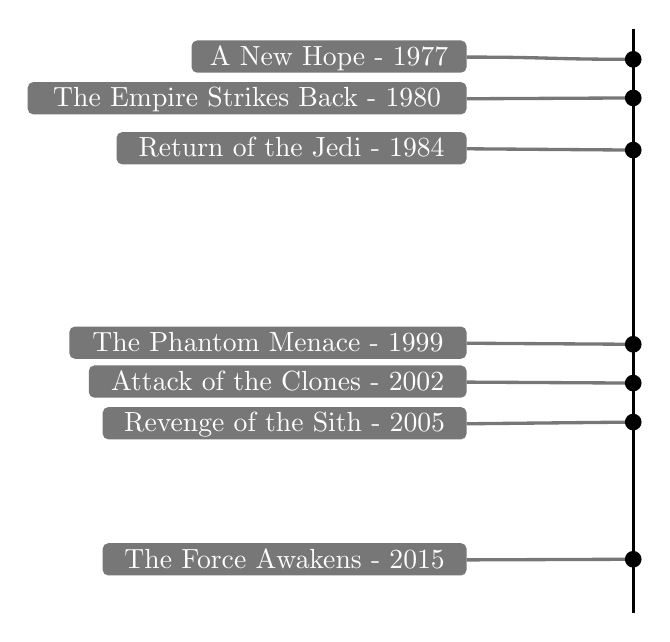
\begin{tikzpicture}[x=1bp,y=-1bp]

% shift for the margin
\begin{scope}[shift={(20, 20)}]
% main layer
\begin{scope}[shift={(360, 0)}]
% axis
\begin{scope}
\draw[very thick] (0, 0) -- (0, 210);
\end{scope}

% link layer
\begin{scope}
\draw[color=linkColorA, very thick] (0.00000000, 10.79589012) .. controls
(-30.00000000, 10.79589012) and (-30.00000000, 10.00000000) .. (-60.00000000, 10.00000000);
\draw[color=linkColorB, very thick] (0.00000000, 24.69708262) .. controls
(-30.00000000, 24.69708262) and (-30.00000000, 25.00000000) .. (-60.00000000, 25.00000000);
\draw[color=linkColorC, very thick] (0.00000000, 43.46624787) .. controls
(-30.00000000, 43.46624787) and (-30.00000000, 43.00000000) .. (-60.00000000, 43.00000000);
\draw[color=linkColorD, very thick] (0.00000000, 113.38106899) .. controls
(-30.00000000, 113.38106899) and (-30.00000000, 113.00000000) .. (-60.00000000, 113.00000000);
\draw[color=linkColorE, very thick] (0.00000000, 127.34614566) .. controls
(-30.00000000, 127.34614566) and (-30.00000000, 127.00000000) .. (-60.00000000, 127.00000000);
\draw[color=linkColorF, very thick] (0.00000000, 141.38788330) .. controls
(-30.00000000, 141.38788330) and (-30.00000000, 142.00000000) .. (-60.00000000, 142.00000000);
\draw[color=linkColorG, very thick] (0.00000000, 190.77086882) .. controls
(-30.00000000, 190.77086882) and (-30.00000000, 191.00000000) .. (-60.00000000, 191.00000000);
\end{scope}

% label layer
\begin{scope}
\begin{scope}[shift={(-159, 4)}]
\fill[color=labelBgColorA, rounded corners=2pt]
(0, 0) rectangle (99, 11.60416) node[midway, yshift=-.75bp, anchor=center, text=labelTextColorA] {\strut \textA};
\end{scope}
\begin{scope}[shift={(-218, 19)}]
\fill[color=labelBgColorB, rounded corners=2pt]
(0, 0) rectangle (158, 11.60416) node[midway, yshift=-.75bp, anchor=center, text=labelTextColorB] {\strut \textB};
\end{scope}
\begin{scope}[shift={(-186, 37)}]
\fill[color=labelBgColorC, rounded corners=2pt]
(0, 0) rectangle (126, 11.60416) node[midway, yshift=-.75bp, anchor=center, text=labelTextColorC] {\strut \textC};
\end{scope}
\begin{scope}[shift={(-203, 107)}]
\fill[color=labelBgColorD, rounded corners=2pt]
(0, 0) rectangle (143, 11.60416) node[midway, yshift=-.75bp, anchor=center, text=labelTextColorD] {\strut \textD};
\end{scope}
\begin{scope}[shift={(-196, 121)}]
\fill[color=labelBgColorE, rounded corners=2pt]
(0, 0) rectangle (136, 11.60416) node[midway, yshift=-.75bp, anchor=center, text=labelTextColorE] {\strut \textE};
\end{scope}
\begin{scope}[shift={(-191, 136)}]
\fill[color=labelBgColorF, rounded corners=2pt]
(0, 0) rectangle (131, 11.60416) node[midway, yshift=-.75bp, anchor=center, text=labelTextColorF] {\strut \textF};
\end{scope}
\begin{scope}[shift={(-191, 185)}]
\fill[color=labelBgColorG, rounded corners=2pt]
(0, 0) rectangle (131, 11.60416) node[midway, yshift=-.75bp, anchor=center, text=labelTextColorG] {\strut \textG};
\end{scope}
\end{scope}

% dots
\begin{scope}
\draw node [circle, inner sep=0pt, minimum size=6bp, 
fill=dotColorA] at (0, 10.795890) {};
\draw node [circle, inner sep=0pt, minimum size=6bp, 
fill=dotColorB] at (0, 24.697083) {};
\draw node [circle, inner sep=0pt, minimum size=6bp, 
fill=dotColorC] at (0, 43.466248) {};
\draw node [circle, inner sep=0pt, minimum size=6bp, 
fill=dotColorD] at (0, 113.381069) {};
\draw node [circle, inner sep=0pt, minimum size=6bp, 
fill=dotColorE] at (0, 127.346146) {};
\draw node [circle, inner sep=0pt, minimum size=6bp, 
fill=dotColorF] at (0, 141.387883) {};
\draw node [circle, inner sep=0pt, minimum size=6bp, 
fill=dotColorG] at (0, 190.770869) {};
\end{scope}

\end{scope}
\end{scope}
\end{tikzpicture}
\end{document}